% Chapter 1

\chapter{Proposal} % Main chapter title

\label{prop} % For referencing the chapter elsewhere, use \ref{Chapter1} 

\lhead{Proposed Approach} % This is for the header on each page - perhaps a shortened title
Considering the fact that energy efficiency is the primary goal of any wireless sensor network application, we have designed DS-MMAC, Dynamic Schedule based MAC protocol for Mobile Wireless sensor network. It should be noted that DS-MMAC is specifically designed for mixed deployment of sensor nodes (mobile and static). It is assumed that a dense random deployment of static nodes is available. This approach is a pure MAC protocol i.e. routing is handled separately. Routing is handled separately using a modified version of AODV \cite{aodv}. Based on our performance evaluation of DS-MMAC, we observe that it performs very under in a mixed deployment scenario with mobile nodes moving at low velocities. The algorithm is explained in detail in the following sections. We have simulated DS-MAC and compared the results against Hybrid MAC \cite{hmac} in Chapter \ref{simulacra}. 

As a continuation of DS-MMAC, we have also designed a Cross Layer Architecture for a strictly mobile sensor network, CA-MOBILE. Unlike DS-MMAC, CA-MOBILE inherently handles routing by forwarding data packets to a node which is closest or potentially close to the base station. The key aspects of this approach are Dynamic Cluster Head Election, Multi-channel Data Transfer and Mutually Beneficial Forwarder Assignment. Inspired by opportunistic routing techniques \cite{exor}\cite{rof}, we have designed CA-MOBILE to forward packets by dynamically choosing a forwarder for each source node, using updated mobility information of the cluster. It should be noted that even though the initial simulation results of CA-MOBILE are promising, It is not yet analyzed w.r.t to all the network parameters (scalability, reliability, packet delivery ratio, energy efficiency). 

\section{DS-MMAC}

We propose a MAC protocol that uses dynamic scheduling to handle the mobile nodes in the network. Each frame is divided into control phase, for managing the mobile nodes, data transfer phase for collecting data from the mobile nodes and routing phase during which the static node forwards the aggregated data to the next node based on an established routing path \cite{aodv}. We employ request-reply mechanism for data transfer, which not only improves the reliability of the data transfer but also serves as a means to inform the mobile nodes about their wake up time during the next frame. The primary goal of our protocol design is to improve energy efficiency by increasing the sleep time of the mobile nodes. The request-reply mechanism also ensures that collision does not happen when a mobile node moves from one virtual cluster \cite{smac} to another. The local schedule maintained by each static node in the network, is designed to be flexible that it keeps on changing based on network traffic and the mobility of the neighbors.

\subsection{Problem Statement and Assumptions}
Accommodating mobile sensor nodes in the sensor network introduces a few challenges for the network protocol designers. Due to the rapid movement of mobile nodes, the topology of the entire network changes every instant. Designing a MAC and/or routing protocol for a network with dynamic topology is a challenging task. An efficient routing algorithm in this case, essentially requires efficient medium access, with minimum packet loss. Contention based algorithms increase the network overhead and also the probability of collision is high. Hence, this scenario requires a TDMA based MAC protocol which dynamically adapts to the changes in the mobile node traffic in the neighborhood.  

We assume that a dense unstructured deployment of static nodes is available in the network for routing data to the base station. It is also assumed that the cluster head possesses the ability to aggregate data before forwarding to the base station.

\subsection{Algorithm}

\subsubsection{Network Initialization}
The first phase of our approach is Network initialization, during which the static nodes in the network exchange timing slots to communicate with each other. This process of offering a TDMA slot to a static node starts from the base station. It should be noted that none of the static nodes start communication with their mobile neighbors before acquiring a routing slot from their parent. The base station starts off the process by sending different timing slots to all its \emph{children} i.e., one hop static neighbors. The children randomly choose a time slot, different from the one offered to them by the base station and enable their one hop static neighbors(grand children). This process continues until all the nodes acquire a routing slot from their parents. Meanwhile, the nodes which are enabled by their parents, start communicating with their mobile neighbors. Once a mobile node starts receiving data from its neighbors, it starts aggregating the data. This aggregated data is forwarded to its parent during the routing slot offered by its parent, which eventually reaches the base station.


The communication with mobile nodes involves two stages : Control Phase and Data phase. Control phase is organized into (i) Discovery Request Phase (ii) Discovery Reply Phase and (iii) Schedule phase, which are explained clearly in the following sections:

%\subsubsection{Control Phase}
Control Phase is organized into (i) Discovery Request Phase, (ii) Discovery Reply Phase and (iii) Schedule phase.

\subsubsection{Discovery Request Phase}
\label{disc_req_phase}
During the start of the frame, the cluster head broadcasts a discovery request packet \emph{disc\_req}. The discovery request packet is an advertisement message broadcasted by the cluster head to inform the mobile nodes in the neighborhood about the cluster. This message contains valuable information regarding the cluster including cluster size and remaining energy. Also, a mobile node receiving this message can estimate the approximate distance between the cluster head and itself, based on the RSSI value acquired from the radio message. It is possible that a mobile node may receive more than one disc\_req message from more than one cluster head. In that case, the mobile node chooses a cluster based on the current cluster size, remaining energy of the cluster head and the distance between the cluster head and itself.

\begin{figure}[h]{} % Inline image example
  \begin{center}
   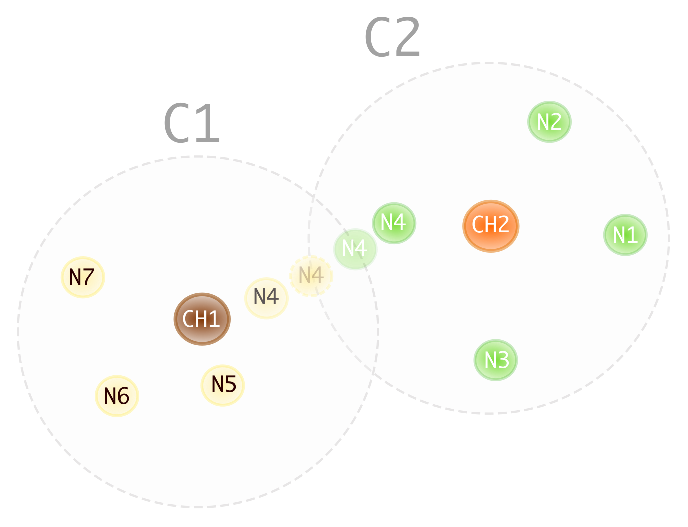
\includegraphics[scale=0.7, natwidth=0.38\textwidth]{scenario01}
	 \caption{A sample scenario}
	 \label{fig:scenario01}
  \end{center}
\end{figure}


\subsubsection{Discovery Reply Phase}
\label{disc_rep_phase}
The Discovery Reply Phase consists of a finite number of slots during which the cluster head listens for Discovery Reply packets \emph{disc\_rep} from the mobile nodes. The mobile node, after choosing a cluster to join, wakes up during a random slot in the Discovery Reply slots and sends a \emph{disc\_rep} packet to the cluster head. The slot selection as mentioned above, is randomly done by the mobile node. The maximum number of these slots is \emph{x} which depends on the node density in the network.

\begin{equation}
	x = m\pi r^2 
	\label{eqn:x}
\end{equation}

$m$: Density of mobile nodes, $r$: Radio coverage radius of static nodes\\

\subsubsection{Schedule Phase}
\label{sched_phase}
Based on the \emph{disc\_req} packets received in the previous section, the cluster head builds a schedule for the mobile nodes to communicate with it. The order of frame access to nodes in this schedule is based on the order of reception of \emph{disc\_rep} packets. The schedule is broadcasted by the cluster head during this phase. It should be noted that any node which issued a join request in this round should be in listen mode during this phase, to receive the schedule packet. 

\begin{figure}[h]{} 
  \begin{center}
    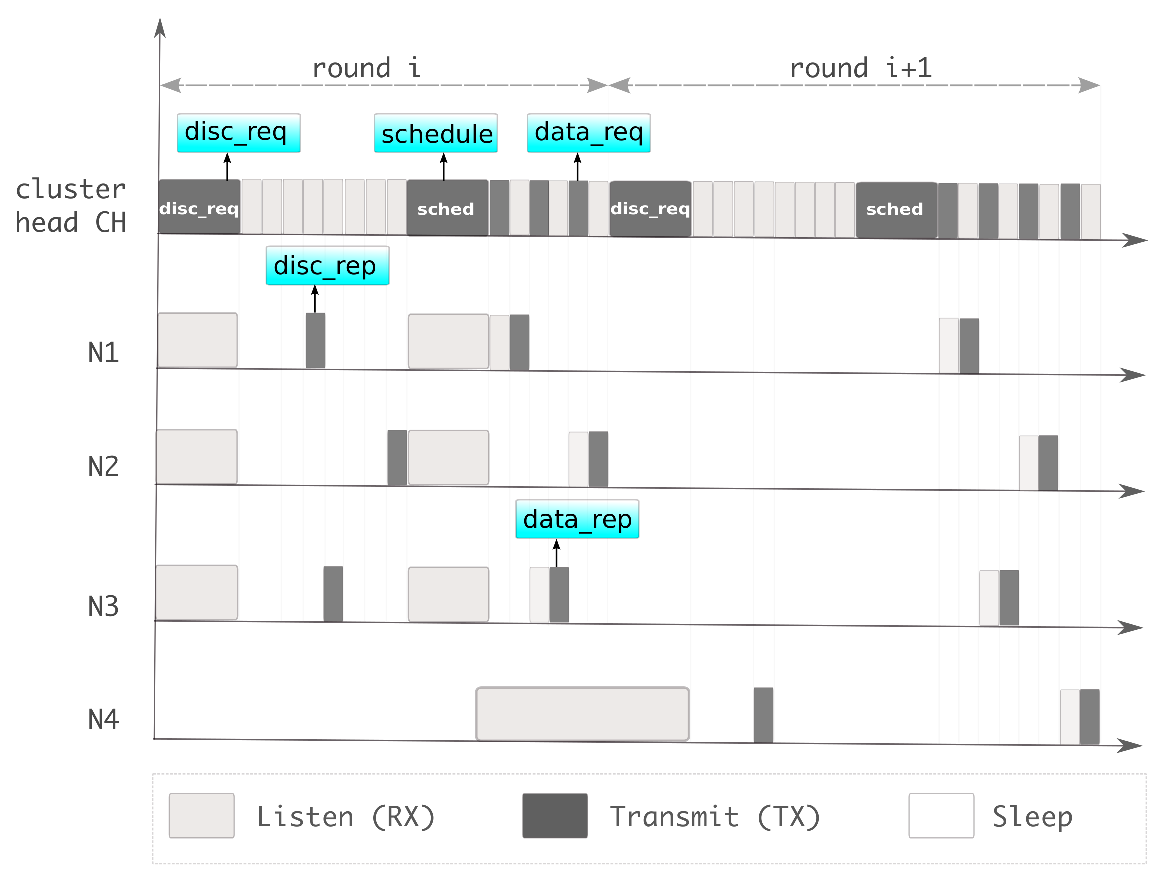
\includegraphics[scale=0.6, natwidth=0.38\textwidth]{timing-dia}
  \end{center}
  \caption{Time line Showing the Cluster head communication}
	\label{fig:timing}
\end{figure}


\subsubsection{Data Phase}
\label{data_phase}

From the schedule message, each mobile node acquires its data slot for communication with the cluster head. The data phase is divided into pairs of \emph{data\_req} and \emph{data\_rep} slots. Each pair serves one mobile node. When a mobile node wakes up during its data slot, it receives a \emph{data\_req} message from the cluster head. The cluster head embeds a time value \emph{$t_1$} in this message, which represents a time in the future (next frame) when the corresponding mobile node should wake up for the next data transfer session. The mobile node after receiving this message sends a \emph{data\_rep} message to the cluster head, set a timer to wake up after \emph{$t_1$} seconds and puts the radio in sleep mode. 

%To understand our approach, let's consider the scenario depicted in figure \ref{fig:scenario}. There are two clusters $C_1$ and $C_2$. Each cluster consists of a few mobile nodes and a cluster head (CH$_1$,CH$_2$). 

Consider the scenario given in figure \ref{fig:scenario01}, where CH$_1$ and CH$_2$ are cluster head of clusters $C1$, $C2$ respectively. Node \emph{$N_4$} moves from $C_1$ to $C_2$. When N4 moves out of the range of CH$_1$, it stops receiving the periodic data request message from CH$_1$. Realizing that it has moved out of cluster $C_1$, N4 switches its radio to listen mode, listening for \emph{disc\_req} packet from other cluster heads.
After waiting a while, it receives a \emph{disc\_req} message from CH$_2$ as shown in figure \ref{fig:timing}. N4 chooses one of the slots in the discovery reply phase to send a \emph{disc\_rep} packet. CH$_2$ adds N4 to the schedule and broadcast the schedule. N4 acquires its data transfer slot timing from the schedule. During its slot, N4 wakes up to receive \emph{data\_req} packet from CH$_2$ and replies to it with a \emph{data\_rep} packet. Using the next data transfer session schedule acquired from the \emph{data\_req} packet, N4 sets a timer and puts its radio in sleep mode.

The algorithm followed by the mobile nodes in our approach is mentioned in Algorithm \ref{algo:mob}. Initially mobile node will switch on its radio to RX state and listens for $disc\_req$ packets from cluster heads. When it receives a $disc\_req$ it binds itself to the cluster head and sends a $disc\_rep$ packet to the cluster head, depicted in lines 2 to 7 in Algorithm \ref{algo:mob}. After which it waits for a $sched$ packet from the cluster head. The mobile node extracts its scheduled slot from $sched$. Based on which, it wakes up and listens for a $data\_req$ packet from the cluster head as given in lines 15,16. Line 17 to 19 describes the data request and response mechanism. The $data\_req$ message also contains the slot during which the mobile node should wake up during the next frame. 


%%%%%%%%%%%%%%%%%%%%%%%%%%%%%%%%%%%%%%%%%%%%%%%%%%%%%%%%%%%%%%%%%%
%\iffalse 
%In this section we will discuss the working of our protocol from a mobile node and from a static node's perspective. 
%
%--- Try framing an algorithm w.r.t the static node. \\
%
%Try framing an algorithm w.r.t the mobile node. \\
%
%Try framing an algorithm w.r.t the timeslot allocation b/w the static node during the network initialization. \\ \\

% ------------------------------------------------------- %
\alglanguage{pseudocode}
\begin{algorithm}[H]
	\caption{From Mobile Node's Perspective}
	\label{algo:mob}
\begin{algorithmic}[1]
	\Procedure {DS-MMAC\_MOBILE}{}%{$P_c$, $N$, $R$, $a$, $\Re$}
	\While{\emph{true}}
%\State toRadioLayer(RX\_STATE)
\If {\emph{receive($disc\_rep$)}}
	\State $CH\gets disc\_rep.source$
	\State $disc\_slot\gets rand()$
	\State \emph{Wake up at $disc\_slot$}
	\State $send(disc\_rep)$
%	\State toRadioLayer(RX\_STATE)
	\If {\emph{receive(Sched)}}
	\For{$i = 0 \rightarrow Sched.node\_count$}
	\If { Sched.node\_id = ADDR }
	\State $data\_slot \gets Schedule[i].slot$
%	\State toRadioLayer(SLEEP\_STATE)
	\State break
	\EndIf
	\EndFor
	\State \emph{Wake up at $data\_slot$}
%	\State toRadioLayer(RX\_STATE)
	\While{\emph{receive(DataReq)}}
	\State $data\_slot \gets DataReq.slot$
	\State $send(DataRep,CH)$
	\State \emph{Wake up at $data\_slot$}
%	\State toRadioLayer(RX\_STATE)
	\EndWhile
	\EndIf
\EndIf
\EndWhile
\EndProcedure
\end{algorithmic}
\end{algorithm}
%\fi

Algorithm \ref{algo:ch} describes our approach from a cluster head's perspective. The cluster head initiates the communication by broadcasting a $disc\_req$ message and then waits for the nodes in its vicinity to respond with a $disc\_rep$ message. The cluster head stores the addresses of the nodes sending the $disc\_rep$ message in a local buffer \emph{boundNodes}. This process is described in lines 3 to 7. Based on the contents of the buffer, the cluster head builds and broadcasts the schedule for this frame. Lines 13 to 20 depicts how the cluster head services the mobile nodes. It should be noted that in each $data\_req$ message, the cluster head embeds the slot information on when the mobile node should wake up during the next frame.





%%%%%%%%%%%%%%%%%%%%%%%%%%%%%%%%%%%%%%%%%%%%%%%%%%%%%%%%%%%%%%%%%%
\alglanguage{pseudocode}
\begin{algorithm}[H]
	\caption{From Cluster Head's Perspective}
	\label{algo:ch}
\begin{algorithmic}[1]
	\Procedure {DS\_MMAC\_MOBILE}{}%{$P_c$, $N$, $R$, $a$, $\Re$}
	\While{\emph{true}}
%\State toRadioLayer(RX\_STATE)
\If {\emph{receive($disc\_req$)}}
	\State $broadcast(disc\_req)$
	\While{receive(disc\_rep)}
		\State \emph{bound\_nodes.add(disc\_rep.source)}
	\EndWhile
	\For{$i = 0 \rightarrow bound\_nodes.size$}
		%\State $sched.node\_id[i] = boundNodes[i]$
		%\State $sched.slot[i] = 2 \into i + FRAME\_SIZE$
		\State \emph{/* add to schedule */}
	\EndFor
	\State \emph{broadcast(sched)}
	\For{$j = 0 \rightarrow bound\_nodes.size$}
		\State $DataReq.slot \gets next\_slot()$
		\State \emph{send(data\_req,bound\_nodes[j]}
		\If {\emph{receive(data\_rep)}}
			\State \emph{store data\_rep}
		\Else\ \emph{boundNodes.remove(j)}
		\EndIf
	\EndFor
\EndIf
\EndWhile
\EndProcedure
\end{algorithmic}
\end{algorithm}
%

The simulation of DS-MMAC s done and the results are compared with Hybrid MAC proposed in \cite{hmac}. A thorough performance evaluation of DS-MMAC is done and it is described in Chapter \ref{simulacra}.


\section{CA-MMAC}
We propose a Cross Layer Architecture for strictly Mobile WSN that uses mobility parameters of nodes to manage data forwarding in the network. Our algorithm organizes the network into clusters based on geographical location of nodes. Cluster information is updated every round. Each cluster consists of a cluster head which is elected using the standard cluster head election mechanism proposed in \cite{leach}. Cluster head re-election is done when the current cluster head finds a more suitable candidate for the task. During each round the cluster head acquires the mobility information(location,velocity) of the cluster members. Based on the collected information, it assigns a forwarder node for each node with data packets to forward. The assignment is designed in such a way that each node is able to complete the data transfer based on the size of data it contains and also considering the location and velocity of the forwarders chosen. We have discussed the assignment problem in depth in Section \ref{assgn_prob}.


\subsection{Problem Statement}

In a fully mobile Wireless Sensor Network, data forwarding from a sensor node to the base station involves a number of challenges. Mobility of nodes leads to a condition where the links established between nodes changes dynamically. Due to the constant change in link quality, the choice the best node to forward data should consider the mobility parameters of the node. The parameters to be considered are the location of the mobile node w.r.t. to the base station and the source(or the current forwarder). This scenario requires an opportunistic routing protocol which assigns forworders to source nodes based on their mobility parameters.

\subsection{Assumptions}
\begin{itemize}
	\item The network consists of a dense random deployment of mobile nodes 
	\item All nodes are aware of their location and their current velocity
	\item Nodes have the ability to aggregate data before forwarding
	\item Location of basestation is fixed and is known to all the nodes
\end{itemize}


\subsection{Assignment Problem}
\label{assgn_prob}
In the figure, all the nodes inside the gray circle belong to a cluster, $C_1$. CH is their cluster head. The cluster head is responsible for managing the data transfer within the cluster. When a node \emph{N1} has data to send to basestation, it sends a \emph{RTS} (Ready To Send) message CH and now, its CH's responsibility to find a suitable node, \emph{$N_i$} for \emph{N1} to forward its data. We need to consider parameters such as the velocity (direction and speed), distance from the base station, distance from the source/sender node and the contact time between N1 and the $N_i$. Contact time is basically the period during which N1 and $N_i$ are within the range of each other. The first part of the problem is to build a model using the given parameters, using which a node's suitability for forwarding data will be quantified. \\

\begin{figure}[h]{} 
  \begin{center}
		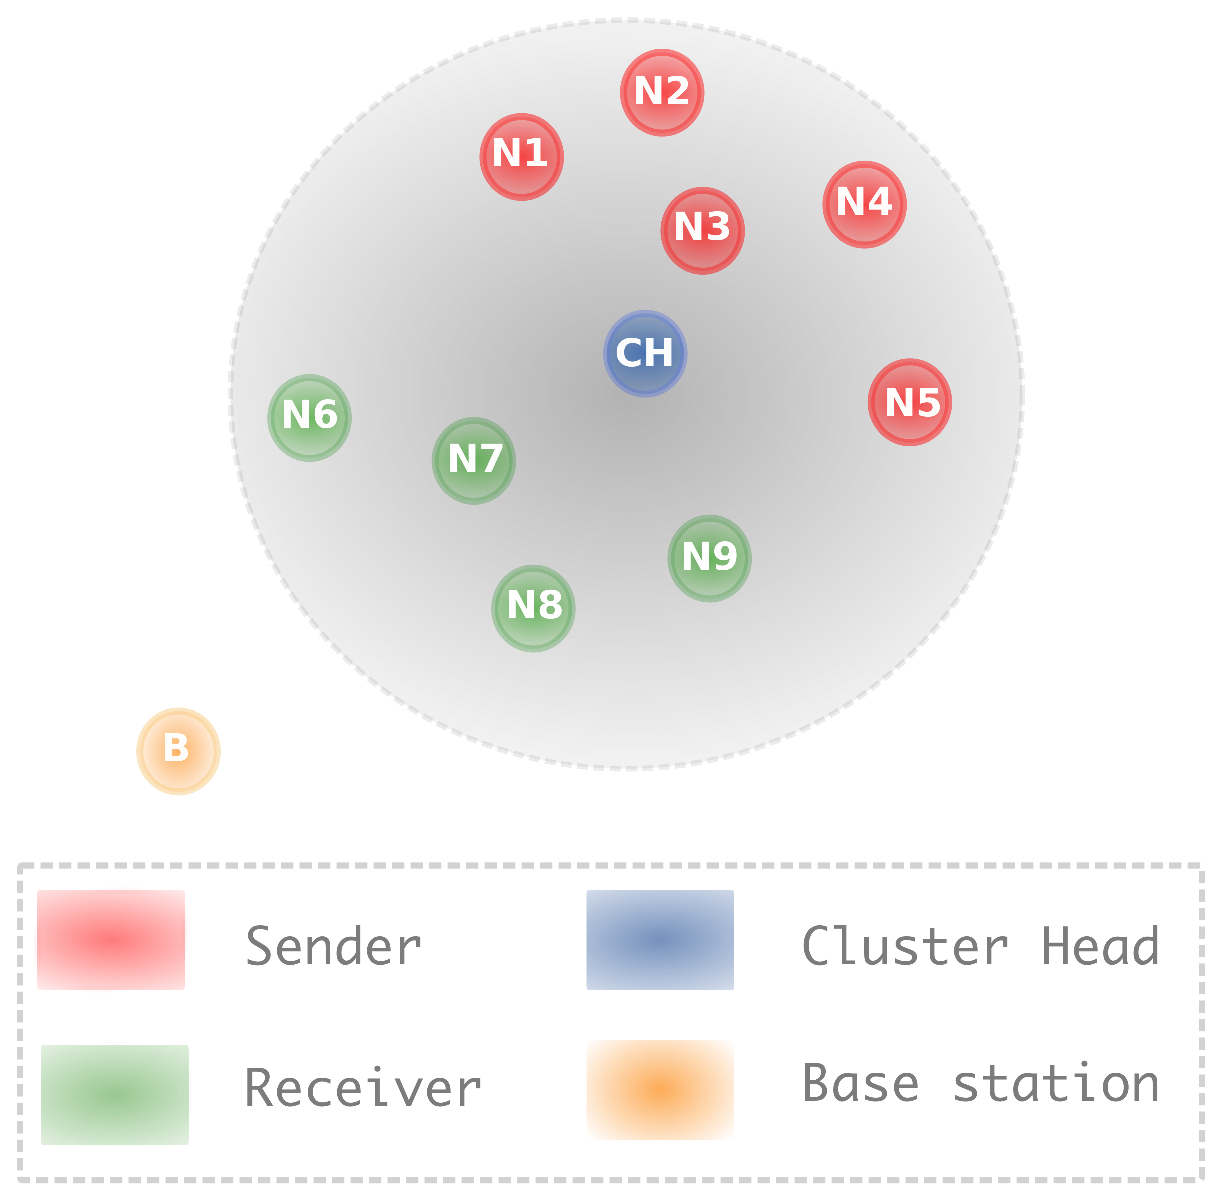
\includegraphics[scale=0.4, natwidth=0.38\textwidth]{ca_mmac_scenario01}
		\caption{Assignment Problem}
	\label{fig:scenario02}
  \end{center}
\end{figure}


The second part of the problem is to decide which destination nodes to assign to which source nodes, based on the model. Assume that the nodes $N_1, N_2, N_3$ and $N_5$ have data to forward to base station and the nodes N6, N7, N8 and N9 are the candidates for destination node. This becomes an assignment problem; which nodes to assign to which nodes?

\subsection{Algorithm}

The first step in our algorithm is Cluster head election. Every node randomly backs off and then broadcasts a $sync$ message. The nodes receiving the $sync$ message, become the cluster members, while the node broadcasting becomes the cluster head. In case of collision of $sync$ message, the process of random back-off and broadcast is repeated. This constitutes the network setup phase. Data gathering and opportunistic forwarding take place in the subsequent phases. Each round in CA-MMAC consists of the following phases: (i) Synchronization (ii) Meta phase (iii) Schedule (iv) Data Phase, which are explained in detail in the following sections. It should be noted that except the data phase, in all the other phases, a common channel is used for communication. 

\subsubsection{Synchronization}
During the synchronization phase, the cluster head broadcasts the $sync$ message, which consists of the cluster information including the cluster size and the centroid of the cluster.  The $sync$ message acts as an advertisement for the new nodes joining the cluster. 

\subsubsection{Meta Phase}
After synchonization, we have meta phase which is split into small slots named meta slots, illustrated in \ref{fig:ca-timing}. The cluster members choose a random meta slot for sending $meta$ packets to the cluster head. The $meta$ packet consists of mobility information of the node incluing current location and velocity. Optionally the cluster members which have data to forward, can embed a Request To Send, $rts$ message along with the $meta$ packet. The cluster head updates the mobility information of the cluster during the meta phase. It then uses this information to decide which node forwards data to which node.

\begin{figure}[h]{} 
  \begin{center}
		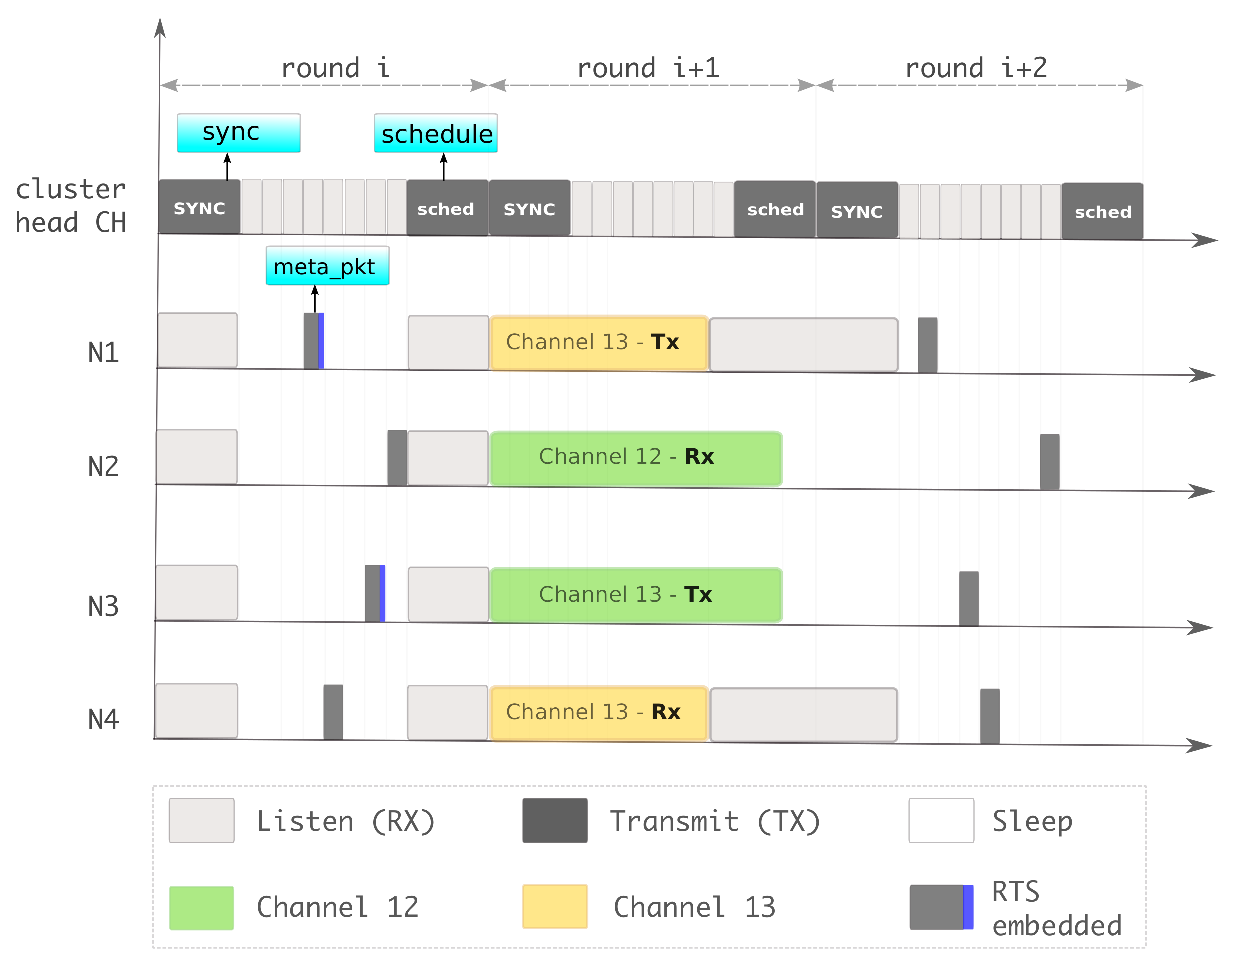
\includegraphics[scale=0.6, natwidth=0.38\textwidth]{ca-timing}
		\caption{Timing Diagram}
	\label{fig:ca-timing}
  \end{center}
\end{figure}


\subsubsection{Schedule}
Baed on the mobility information of the cluster, the cluster head first calculates the distance between each node and the centeroid and the velocity of nodes and decides if the cluster needs a new cluster head. If it chooses a new cluster head, it embeds this message along with the $sched$ packet.  The nodes receiving this message will become aware of the new cluster head, and wait for the next $sync$ message from the newly chosen cluster head, after the end of this frame. The schedule basically consists of data pairs and data channels. The cluster head dynamically chooses a forwarding node for each source node based on the assignment algorithm explained in \ref{assgn_prob}. It also assigns an unique channel over which the data transfer between the corresponding data pair is intended to occur. The nodes receiving the $sched$ message, change their local cluster head variable to the new cluster head's id, in case the cluster head has also sent a new cluster head along with the schedule. By iterating through the schedule, the cluster member comes to know about its data pair and starts data transfer on the assigned channel.

\subsubsection{Data Phase}
The data transfer is designed to include acknowledgement, \emph{ACK} for higher reliability. The receiver keeps track of the RSSI (Receiver Signal Strength) of the data packets sent by the sender, based on which an approximate distance between them is calculated. If this distance crosses a threshold, the receiver sends a \emph{NACK} message to the sender in place of \emph{ACK} Upon receiving the \emph{NACK} message, the sender stops the data transfer and goes to sleep. It continues the data forwarding during the next round, when the cluster head assigns a new forwarding node to it.\\

\alglanguage{pseudocode}
\begin{algorithm}[H]
	\caption{CA-MOBILE : Algorithm}
	\label{algo:ca-mobile}
\begin{algorithmic}[1]
	\Procedure {CA\_MOBILE}{}%{$P_c$, $N$, $R$, $a$, $\Re$}
	\State \emph{/* Random Back-Off */}
	\If {\emph{receive(sync)}}
	% cluster member
	\State $cluster\_head \gets sync.source$
	\While{\emph{true}}
		\State $meta\_slot \gets rand()$
		\State \emph{Wake up at $meta\_slot$}
		\State $meta.mob\_vector \gets self\_mob\_vector()$
		\If {\emph{hasData()}}
			\State $meta.rts \gets true$
		\EndIf
		\State $send(meta)$
		\If {\emph{receive(sched)}}
		\For{$j = 0 \rightarrow sched.node\_count$}
			\If { sched.node\_id = SELF }
				\State $data\_pair \gets sched[i].data\_pair$
				\State $data\_channel \gets sched[i].data\_channel$
			\EndIf
		\EndFor
		\State \emph{/* Switch to data\_channel */}
		\State \emph{/* Initiate data transfer */}
		\EndIf
		\State {\emph{receive(sync)}}
	\EndWhile
	\Else
	\While{\emph{true}}
		\State $broadcast(sync)$
		\While{receive($meta$)}
			\State \emph{bound\_nodes.add(meta.source)}
			\State \emph{mobility\_vector.add(meta.mob\_vector)}
		\EndWhile
		\State $new\_cluster\_head \leftarrow min(boundNodes,centroid)$
		\State $sched.embed(new\_cluster\_head)$
		\For{$i = 0 \rightarrow bound\_nodes.size$}
			\State \emph{/* Assign data pair, data channel, add to schedule */}
		\EndFor
		\State \emph{broadcast(sched)}
			\Else\ \emph{boundNodes.remove(j)}
	\EndWhile
	\EndIf
\EndProcedure
\end{algorithmic}
\end{algorithm}
